\chapter{Détermination des paramètres pour des simulations} \label{ann:parametrage}
L'objectif est de ce placer dans le cas binaire, ainsi on pose $\phi_B^k = \phi_{B}^{eq,k}$ et $\phi_A^k = \phi^{k}$
.\begin{align*} 
\Omega^{\star} &= P^{disp} \times P^{cont} \\ 
& = \left(\phi_{}-\phi_{}^{eq,disp}\right)^2\left(\phi_{}-\phi_{}^{eq,cont}\right)^2\left[ \left(\frac{\co{\theta^{disp}}}{a^\alpha}\right)^2 + \left(\frac{\sinus{\theta^{disp}}}{b^\alpha}\right)^2  \right]
\left[ \left(\frac{\co{\theta^{cont}}}{a^\beta}\right)^2 + \left(\frac{\sinus{\theta^{cont}}}{b^\beta}\right)^2  \right]
\end{align*}
Par soucis de simplification on définit une constante $\Lambda$ tel que : 
\begin{equation}
\Lambda^2 = \left[ \left(\frac{\co{\theta^{disp}}}{a^\alpha}\right)^2 + \left(\frac{\sinus{\theta^{disp}}}{b^\alpha}\right)^2  \right]
\left[ \left(\frac{\co{\theta^{cont}}}{a^\beta}\right)^2 + \left(\frac{\sinus{\theta^{cont}}}{b^\beta}\right)^2  \right]
\end{equation}
On rappelle la formule reliant la tension de surface et le paramètre d'ordre dans le cas binaire : 
\begin{equation}
\sigma = \int_0^L\kappa^{bin}\left(\frac{d\phi}{dz}\right)^2dz
\end{equation}
Ainsi on peut écrire :
\begin{align}
\sigma & = \sqrt{2\kappa\lambda}\int_{\phi^{disp,eq}}^{\phi^{cont,eq}}\sqrt{\Omega^{\star}}d\phi \\
\nonumber	& = \sqrt{2\kappa\lambda}\int_{\phi^{disp,eq}}^{\phi^{cont,eq}}\left(\phi_{}-\phi_{}^{eq,disp}\right)\left(\phi_{}-\phi_{}^{eq,cont}\right)\Lambda d\phi \\
\nonumber	& = \sqrt{2\kappa\lambda}\int_{\phi^{disp,eq}}^{\phi^{cont,eq}}\left\{\phi_{}^2 -\phi_{} \left(\phi^{eq,disp} +\phi^{eq,cont} \right) + \phi^{eq,disp}\phi^{eq,cont}\right\}\Lambda d\phi \\
\nonumber	&  = \sqrt{2\kappa\lambda} \Lambda \left[\cfrac{\phi^3}{3} - \cfrac{\phi^2}{2} \left(\phi^{eq,disp} +\phi^{eq,cont} \right) +\phi \phi^{eq,disp}\phi^{eq,cont}      \right]_{\phi^{disp,eq}}^{\phi^{cont,eq}}
\end{align}
Dans les cas où les composant ne sont pas totalement miscible/immiscible on obtient un résultat de la forme :
\begin{multline}
	\sigma=  \sqrt{2\lambda\kappa} \Lambda\biggl(\cfrac{\left(\phi^{eq,cont}\right)^3-\left(\phi^{eq,disp}\right)^3}{3} -\frac{1}{2} \left(\left(\phi^{eq,cont}\right)^2-\left(\phi^{eq,disp}\right)^2  \right)  \left(\phi^{eq,disp} +\phi^{eq,cont} \right) \\ +\left(\phi^{eq,cont}-\phi^{eq,disp}\right)\phi^{eq,disp}\phi^{eq,cont}\biggl)
\end{multline}
Ainsi on pose : 
\begin{multline}
	\xi_1 = \bigg|\Lambda\bigg(\cfrac{\left(\phi^{eq,cont}\right)^3-\left(\phi^{eq,disp}\right)^3}{3} -\frac{1}{2} \left(\left(\phi^{eq,cont}\right)^2-\left(\phi^{eq,disp}\right)^2  \right) \left(\phi^{eq,disp}  +\phi^{eq,cont} \right) \\ +\left(\phi^{eq,cont}-\phi^{eq,disp}\right)\phi^{eq,disp}\phi^{eq,cont}\bigg)\bigg|
\end{multline}
On rappelle également la définition de l'épaisseur d'interface :
\begin{align}
\epsilon&= \cfrac{\phi_{}^{eq,cont}-\phi_{}^{eq,dis}}{\max\left(\cfrac{d\phi_{}}{dz}\right)}
\\
&=\sqrt{\frac{\kappa}{2\lambda}}\frac{\phi^{eq,cont}-\phi^{eq,dis}}{\max\left(\sqrt{\Omega^{\star}}\right)}
\end{align}
Cette définition peut s'observer géométriquement :
\begin{figure}[H]
	\centering
	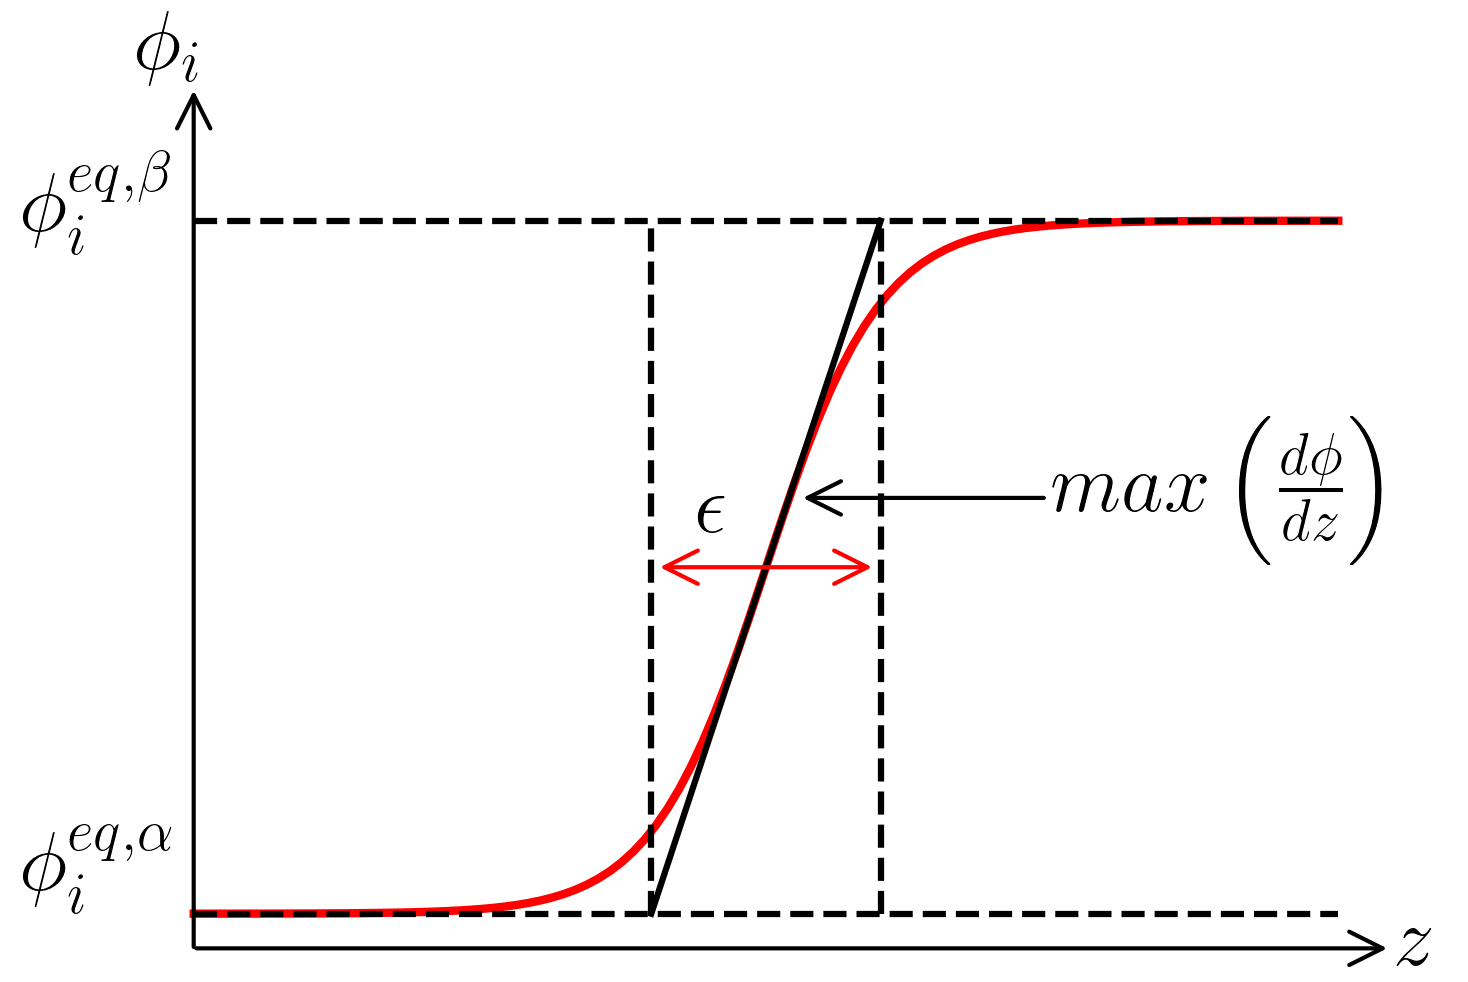
\includegraphics[width=0.3\linewidth]{figure/fig_interface}
	\caption{Définition de l'interface choisie}
	\label{fig:figinterface}
\end{figure}

Ainsi on pose :
\begin{align}
\xi_2&=\frac{\phi^{eq,cont}-\phi^{eq,dis}}{\max\left(\sqrt{\Omega^{\star}}\right)} \\
& = \cfrac{\phi^{eq,cont}-\phi^{eq,dis}}{\max({\left(\phi_{}-\phi_{}^{eq,disp}\right)\left(\phi_{}-\phi_{}^{eq,cont}\right)\Lambda})}
\end{align}

Finalement les coefficients de gradient et facteur d'agrandissement sont obtenus tel que : 
\begin{equation}
\kappa = \frac{\sigma \epsilon}{\xi_1 \xi_2}
\label{eq:kappa_potentiel_ternaire_}
\end{equation}
\begin{equation}
\lambda=\frac{\xi_2 \sigma}{2\epsilon\xi_1}
\label{eq:parametre_upscaling_potentiel_ternaire_}
\end{equation}